\chapter{PENGUJIAN DAN ANALISIS}
\label{chap:pengujiananalisis}

% Ubah bagian-bagian berikut dengan isi dari pengujian dan analisis

\section{Pengujian Model Bahasa}
Berikut hasil dari pengujian model bahasa dalam menghasilkan aksi robot
\begin{figure} [H] \centering
  % Nama dari file gambar yang diinputkan
  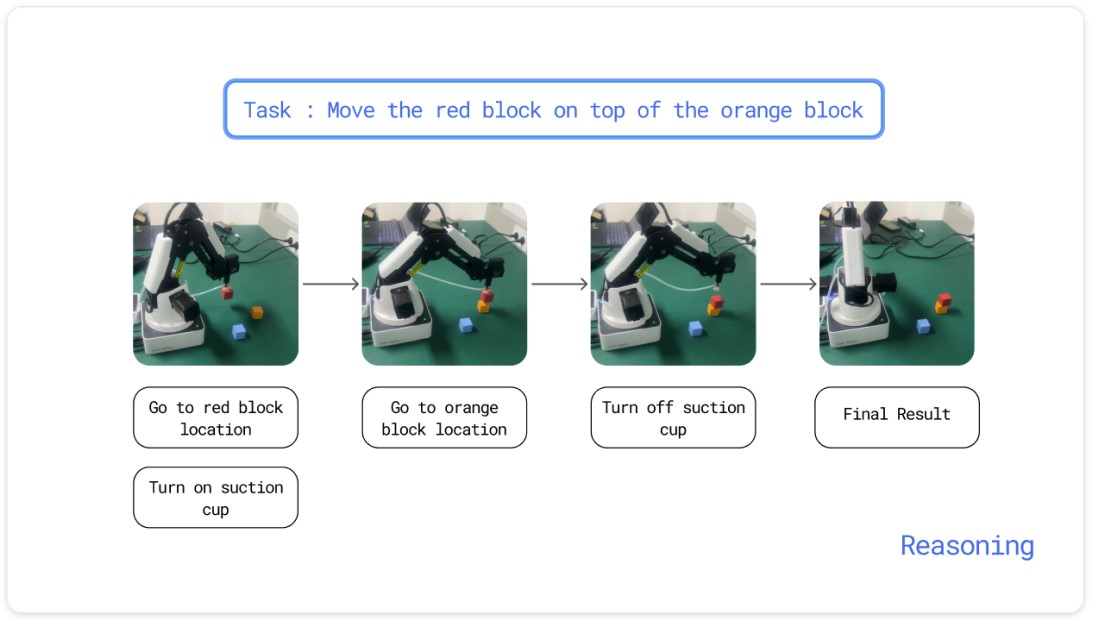
\includegraphics[scale=0.45]{gambar/uji_res.jpg}
  % Keterangan gambar yang diinputkan
  \caption{Uji Reasoning}
\end{figure}

\begin{figure} [H] \centering
  % Nama dari file gambar yang diinputkan
  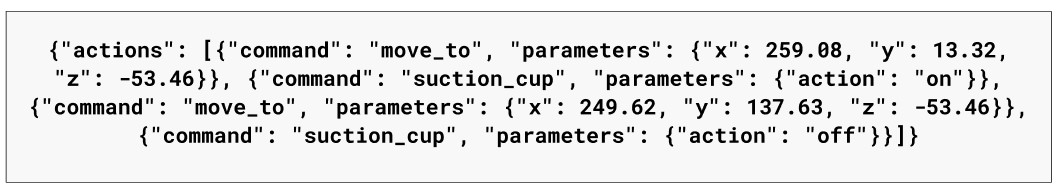
\includegraphics[scale=0.5]{gambar/js1.jpg}
  % Keterangan gambar yang diinputkan
  \caption{Hasil JSON Reasoning}
\end{figure}


\begin{figure} [H] \centering
  % Nama dari file gambar yang diinputkan
  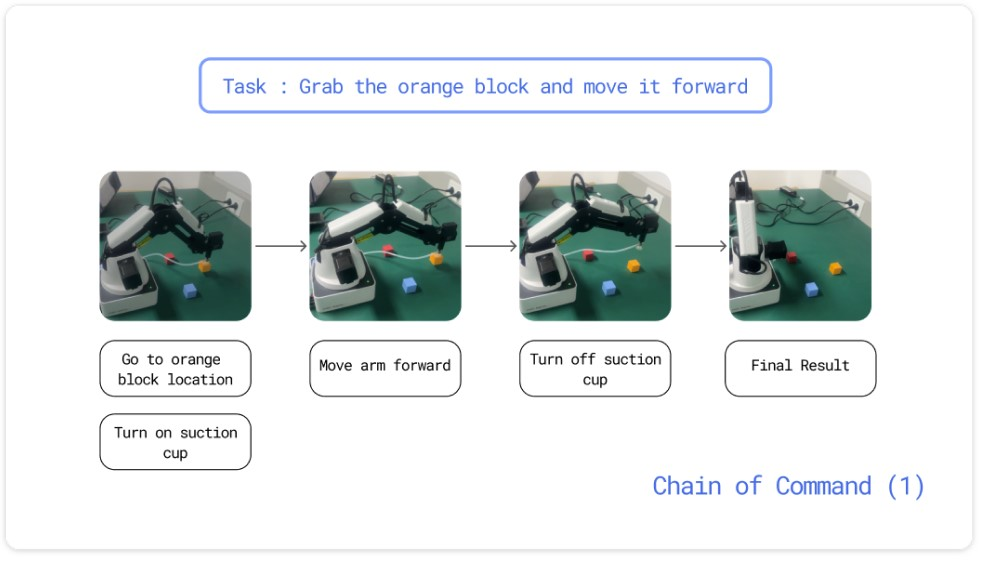
\includegraphics[scale=0.45]{gambar/ujicoc.jpg}
  % Keterangan gambar yang diinputkan
  \caption{Uji Chain of Command}
\end{figure}

\begin{figure} [H] \centering
  % Nama dari file gambar yang diinputkan
  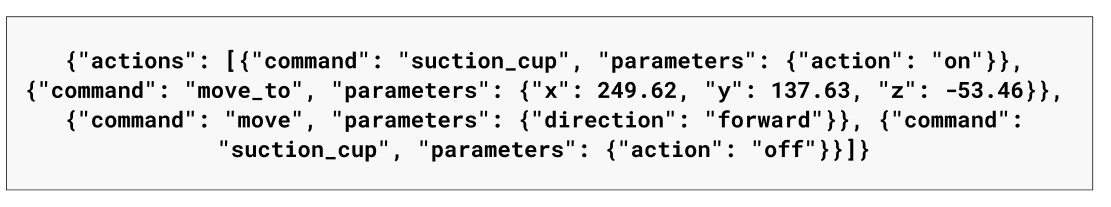
\includegraphics[scale=0.5]{gambar/coc.jpg}
  % Keterangan gambar yang diinputkan
  \caption{Hasil JSON Chain of Command}
\end{figure}



\begin{figure} [H] \centering
  % Nama dari file gambar yang diinputkan
  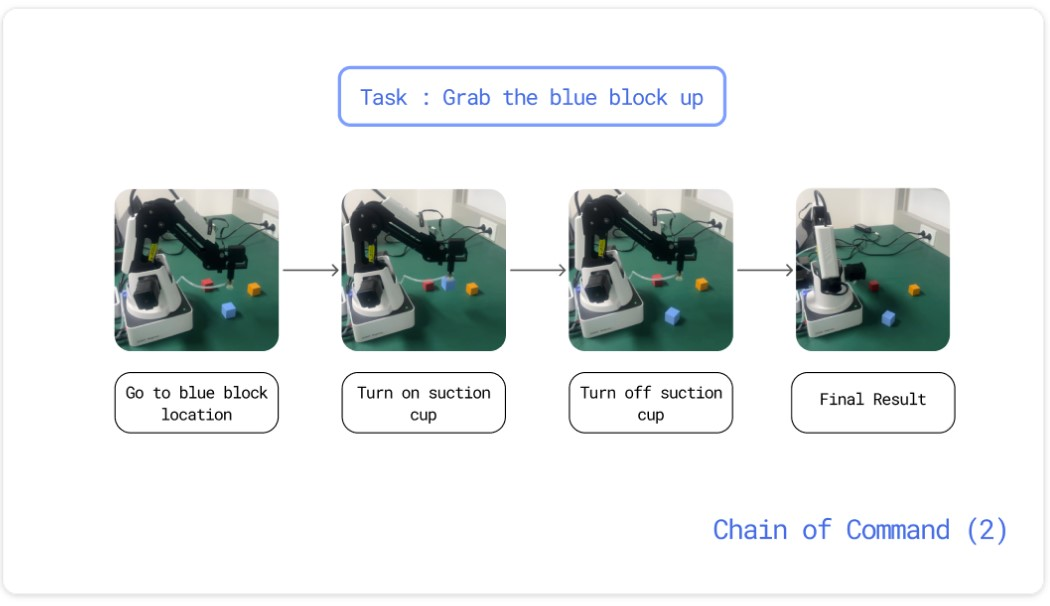
\includegraphics[scale=0.6]{gambar/ujicoc2.jpg}
  % Keterangan gambar yang diinputkan
  \caption{Uji Direct Command}
\end{figure}

\begin{figure} [H] \centering
  % Nama dari file gambar yang diinputkan
  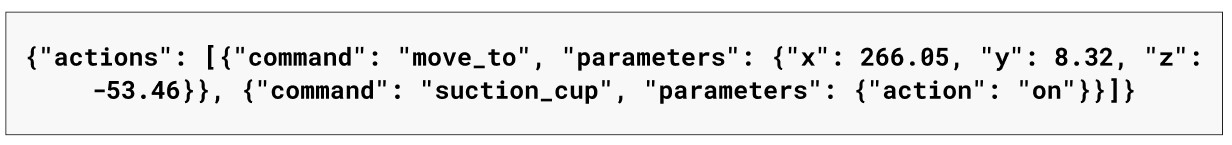
\includegraphics[scale=0.5]{gambar/dc1.jpg}
  % Keterangan gambar yang diinputkan
  \caption{Hasil JSON Direct Command}
\end{figure}

\begin{figure} [H] \centering
  % Nama dari file gambar yang diinputkan
  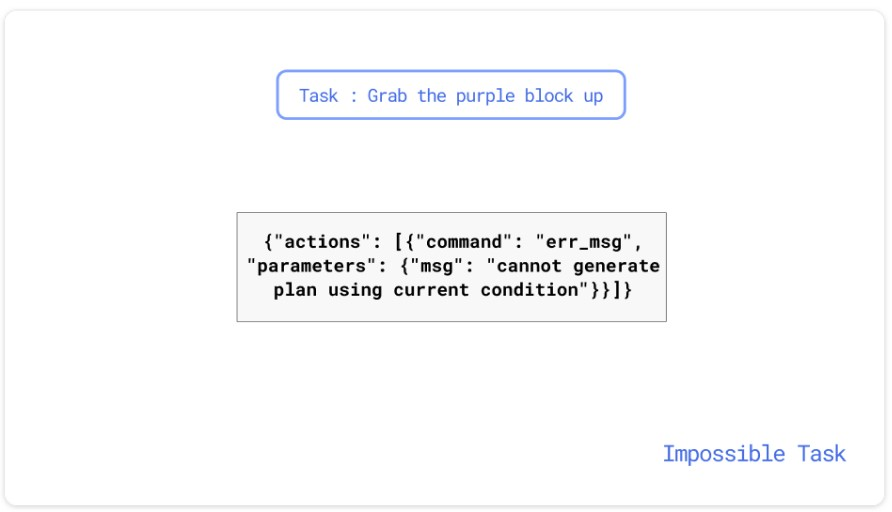
\includegraphics[scale=0.6]{gambar/ujipos.jpg}
  % Keterangan gambar yang diinputkan
  \caption{Uji Impossible Task}
\end{figure}



\section{Metrik Pengujian}
\label{sec:analisis pengujian}

Berikut hasil dari pengujian metrik dibandingkan dengan model Gemma-7b-it dan juga GPT3.5. Dari hasil tersebut model bahasa yang sudah di finetuned memiliki performa terbaik dibandingkan model yang tidak mengalami finetuned dengan jumlah parameter yang lebih besar. Hal ini dapat disebabkan karena kurangnya adaptasi model bahasa terhadap dataset untuk bagian menghasilkan rencana aksi robotika.

\begin{figure} [H] \centering
  % Nama dari file gambar yang diinputkan
  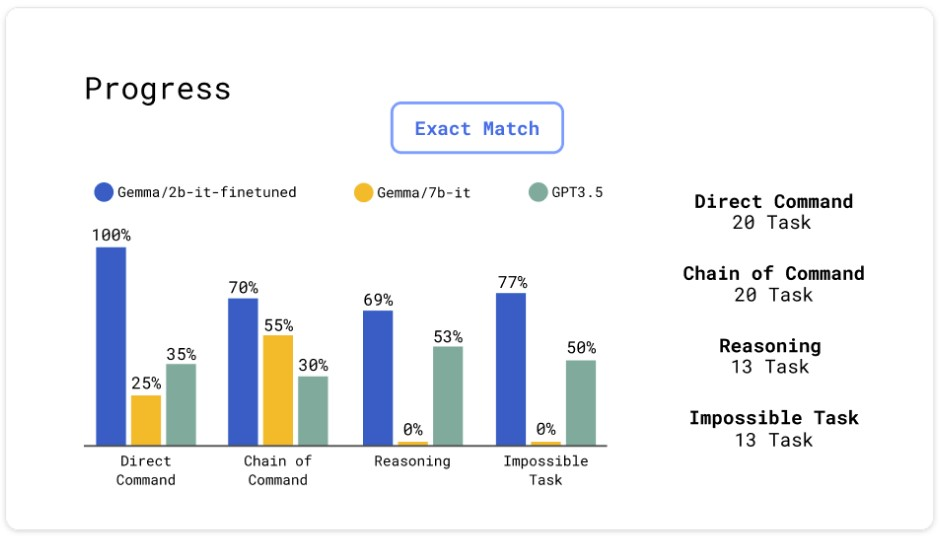
\includegraphics[scale=0.7]{gambar/metrik.jpg}
  % Keterangan gambar yang diinputkan
  \caption{Tuning}
\end{figure}

Direct command adalah tugas di mana LLM harus mengikuti instruksi yang diberikan secara langsung. Dalam tugas ini, model terbaik adalah model yang sudah di tuned yaitu mencapai 100 persen tingkat kecocokan. Hal ini menunjukkan bahwa semua model LLM mampu memahami dan mengikuti instruksi yang diberikan secara langsung dengan sempurna.

Chain of command adalah tugas di mana LLM harus mengikuti serangkaian instruksi yang diberikan secara berurutan. Dalam tugas ini, Gemma/2b-it-finetuned mencapai skor tertinggi, yaitu 70 persen. Hal ini menunjukkan bahwa model ini mampu memahami dan mengikuti serangkaian instruksi dengan baik. Model Gemma/7b-it dan GPT3.5  mencapai skor yang lebih rendah, yaitu 55 persen  dan 30 persen berturut-turut. Hal ini menunjukkan bahwa model-model ini masih memiliki kesulitan dalam memahami dan mengikuti serangkaian instruksi dengan sempurna.

Reasoning adalah tugas di mana LLM harus menggunakan penalarannya untuk menyelesaikan suatu masalah. Dalam tugas ini, Gemma/2b-it-finetuned dan GPT3.5 mencapai skor tinggi, yaitu sebesar 69 persen dan 53 persen. Sedangkan Gemma/7b-it memiliki skor yang sangat rendah. Hal ini menunjukkan bahwa model yang telah tuning mampu menggunakan penalarannya dengan baik untuk menyelesaikan permasalahan yang langkahnya tidak secara eksplisit ditunjukkan oleh input user.

Impossible task adalah tugas yang tidak mungkin diselesaikan oleh LLM karena tidak memenuhi batasan lingkungan atau command. Dalam tugas ini, model Gemma/2b-it-finetuned mencapai skor terbaik yaitu 77 persen disusul oleh GPT3.5 yaitu sebesar 50 persen. Hal ini menunjukkan bahwa model mampu memahami batasan lingkungan nyata dalam menghasilkan rencana aksi robotik.

